Este capítulo é dedicado ao desenvolvimento do primeiro algoritmo de \textit{Data Augmentation}, onde são geradas RIRs simuladas (RIRSM)
a partir de RIRs originais (RIRO). São observados os parâmetros de razão Direto-Reverberante (DRR) e tempo de reverberação (T60), que são
inferidos com base em uma RIRO e que serão manipulados pelo algoritmo para gerar RIRs que vão representar modelos acústicos diferentes.

\begin{figure} [H]
    \centering
    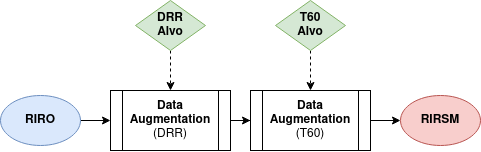
\includegraphics[scale=0.6]{flow-rir-aug.png}
    \caption{Fluxo de procedimentos para gerar a RIRSM.}
    \label{fig:flow-rir-aug}
\end{figure}

Este trabalho é uma implementação dos passos demonstrados no artigo \cite{RIR_Data_Aug}. A figura \ref{fig:flow-rir-aug} especifica 
o fluxo de procedimentos implantados por este algoritmo, onde a DRR e T60 alvos são os valores escolhidos pelo usuário que determinam
as características da RIRSM. 

Antes de explicar os métodos usados, é necessário definir duas funções; 

\begin{align} 
    h_e(t) &= 
    \begin{cases} \label{eqn:rir-early}
        h(t), & t_d-t_0 \le t \le t_d+t_0 \\
        0, & \text{caso contrário,}
    \end{cases} \\
    h_l(t) &= 
    \begin{cases} \label{eqn:rir-late}
        h(t), & t < t_d - t_0 \\
        h(t), & t > t_d + t_0 \\
        0, & \text{caso contrário,}
    \end{cases}
\end{align}

\noindent
onde $t$ representa o tempo discreto, $t_d$ o tempo que as ondas sonoras diretas, ou seja, sem reflexão, levam da fonte até o destino de gravação,
$t_0$ a janela de tolerância, neste caso definida com o valor 2,5 ms \cite{RIR_Data_Aug}, 
$h(t)$ uma RIR, $h_e(t)$ a resposta adiantada e $h_l(t)$ a resposta atrasada.
Neste algoritmo, $t_d$ é determinado da forma:

\begin{align} \label{eqn:t_d}
    %t_d = t_{max},\ onde \ \ h(t_{max}) = max(h(t))
    \begin{cases}
        t_d = t_{max},\\
        t_{max}, \ onde \ h(t_{max}) = max(h(t))
    \end{cases}
    .
\end{align}

\section{Razão Direto-Reverberante (DRR)}

A DRR representa a razão entre a energia sonora da resposta ao impulso que atinge o alvo diretamente e a energia reverberante,
ou seja, que é refletida pelas paredes do ambiente fechado. Este parâmetro é definido da forma:

\begin{equation} \label{eqn:DRR_def}
    DRR_{dB} = 10 \log_{10} \left( \frac{\sum_t h^2_e(t)}{\sum_t h^2_l(t)} \right).
\end{equation}

Para obter a DRR alvo desejada, aplica-se um fator de ganho escalar $\alpha$ na resposta adiantada $h_e(t)$.
De acordo com \cite{RIR_Data_Aug}, para evitar descontinuidades durante o cálculo do fator $\alpha$, refatora-se a
resposta adiantada em duas parcelas, uma que representa a janela direta no pico de intensidade de $h(t)$ e outra
que representa uma janela de resíduo de $h_e(t)$ formando, assim,

\begin{equation} \label{eqn:new-h_e}
    h'_e(t) = \alpha w_d(t) h_e(t) + [1 - w_d(t)]h_e(t),
\end{equation}

\noindent
onde $w_d(t)$ representa uma janela de Hann de duração de 5 ms, pois a janela de tolerância $t_0 = 2,5$ ms.
Substituindo na equação \ref{eqn:DRR_def} $h'_e(t)$ por $h'_e(t)$ e ajustando com a expressão \ref{eqn:new-h_e}, obtem-se
a seguinte equação quadrática;

\begin{equation} \label{eqn:DRR_quad_eqn}
    \begin{aligned} 
        \alpha^2 \sum_t w^2_d(t) h^2_e(t) +
        2 \alpha \sum_t [1 - w_d(t)] w_d(t) h^2_e(t) + \\
        \sum_t [1 - w_d(t)]^2 h^2_e(t) -
        10^{DRR_{dB}/10} \sum_t h^2_l(t)
        = 0
    \end{aligned}    
    ,
\end{equation}

O $\alpha$ desejado será a raiz de maior valor. 
Uma ressalva deste procedimento é que se deve atentar para não escolher um $DRR_{dB}$ que não seja muito menor que o original,
pois após a transformação do $h_e(t)$ para $h'_e(t)$, dependendo do valor de $\alpha$, é possível incidir em um caso onde
$max(h'_e(t)) < max(h_l(t))$, tornando a RIRSM impraticável.

% ### TODO: [FIGURA] Exemplo de RIR antes/depois de fazer DA DRR.
% ### TODO: [FIGURA] Exemplo de RIR com o problema do corte.

\section{Tempo de Reverberação (T60)}

\section{Comparação entre RIR real e simulada}